%\pdfoutput=1
\documentclass[12pt,a4paper,reqno]{amsart}
\newcommand\hmmax{0}
\newcommand\bmmax{0}
\usepackage{amssymb}
\usepackage{amscd}
\usepackage[pdftex,pdfpagelabels]{hyperref}
\usepackage{enumerate}
%\usepackage{psfig}
\usepackage{graphicx}
%\usepackage{showkeys}  
\usepackage{siunitx}
\usepackage{tikz-cd}
\usepackage{stix}
\usepackage{bm}
\DeclareMathAlphabet\mathbfcal{LS2}{stixcal}{b}{n}
\numberwithin{equation}{section}

%\usepackage{mathabx}


\usepackage{mathtools}%                  http://www.ctan.org/pkg/mathtools
\usepackage[tableposition=top]{caption}% http://www.ctan.org/pkg/caption
\usepackage{booktabs,dcolumn}%           http://www.ctan.org/pkg/dcolumn + http://www.ctan.org/pkg/booktabs

% Lighter notation.
%\newcommand*\mc[1]{\multicolumn{1}{c}{#1}}
%\newcommand*\tupref[2]{\href{http://math.mit.edu/~primegaps/tuples/admissible_#1_#2.txt}{\num{#2}}}



%\DeclareMathOperator*\Kl{Kl} (commented because yield bad display for  \Kl_q %replaced with \newcommand... )
%\DeclareMathOperator*\FT{FT} (commented because yield bad display for \FT_q
%replaced with \newcommand...)

\DeclareMathOperator*\swan{swan}
\DeclareMathOperator*\cond{cond}
\DeclareMathOperator*\Gal{Gal}

\newcommand{\FT}{\mathrm{FT}}
\newcommand{\Kl}{\mathcal{K}\ell}
% Setup for ``caption''.
%\DeclareCaptionLabelSeparator{separation}{:\quad}
%\captionsetup{
	%font=small,
	%labelfont=sc,
	%labelsep=separation,
	%width=0.8\textwidth
	%}

\DeclareFontFamily{OT1}{rsfs}{}
\DeclareFontShape{OT1}{rsfs}{n}{it}{<-> rsfs10}{}
\DeclareMathAlphabet{\mathscr}{OT1}{rsfs}{n}{it}

\addtolength{\textwidth}{3 truecm}
\addtolength{\textheight}{1 truecm}
\setlength{\voffset}{-.6 truecm}
\setlength{\hoffset}{-1.3 truecm}

\theoremstyle{plain}

\newtheorem{theorem}{Theorem}[section]
%\newtheorem{theorem}[theorem]{Theorem}
\newtheorem{proposition}[theorem]{Proposition}
\newtheorem{lemma}[theorem]{Lemma}
\newtheorem{axiom}[theorem]{Axiom}
\newtheorem{corollary}[theorem]{Corollary}
\newtheorem{conjecture}[theorem]{Conjecture}
\newtheorem{heuristic}[theorem]{Heuristic}
\newtheorem{principle}[theorem]{Principle}
\newtheorem{question}[theorem]{Question}
\newtheorem{claim}[theorem]{Claim}

\theoremstyle{definition}

%\newtheorem{roughdef}[subsection]{Rough Definition}
\newtheorem{definition}[theorem]{Definition}
\newtheorem{remark}[theorem]{Remark}
\newtheorem{remarks}[theorem]{Remarks}
\newtheorem{example}[theorem]{Example}
\newtheorem{examples}[theorem]{Examples}
%\newtheorem{problem}[subsection]{Problem}
%\newtheorem{question}[subsection]{Question}

\renewcommand\P{\mathbf{P}}
\newcommand\E{\mathbf{E}}
\newcommand\Var{\mathbf{Var}}
\newcommand\R{\mathbb{R}}
\newcommand\Z{\mathbb{Z}}
\newcommand\N{\mathbb{N}}
\newcommand\n{\mathbf{n}}
\renewcommand\a{\mathbf{a}}
\renewcommand\b{\mathbf{b}}
\renewcommand\j{\mathbf{j}}
\renewcommand\k{\mathbf{k}}
\renewcommand\v{\mathbf{v}}
\renewcommand\t{\mathbf{t}}
\renewcommand\r{\mathbf{r}}
\renewcommand\l{\mathbf{l}}
\newcommand\X{\mathbf{X}}
\newcommand\T{\mathbf{T}}
\newcommand\Y{\mathbf{Y}}
\newcommand\A{\mathbf{A}}
\newcommand\W{\mathbf{W}}
\newcommand\C{\mathbb{C}}
\newcommand\Q{\mathbb{Q}}
\renewcommand\Re{{\operatorname{Re}}}
\renewcommand\Im{{\operatorname{Im}}}
\newcommand\eps{\varepsilon}
\newcommand\deriv{\zeta}
\newcommand\zero{\lambda}

\renewcommand{\mod}{\bmod}

\parindent 0mm
\parskip   5mm 


\begin{document}
	
	\title{From Prime-Gap-Inequality to Goldbach-Triangle}
	
	\author{Jianglin Luo}
	\address{WangYueHu Community 1-pian 7-dong, Changsha, China 230026.}
	\email{cody@ustc.edu}
	
	
	\subjclass[2020]{11N05, 40A05}
	
	\begin{abstract}
		The i-th prime gap $p_{i+1}-p_{i}\leq i$. This follows from 
		Prime-Factor-Lemma: We can dispatch distinct prime factors for 
		$\{p_i,p_i+1,\dots,p_{i+1}-1\}$. 
		
		XXX: A feasible dispatching algorithm 
		is to take the significant prime factor $spf(n)$ or the historical prime factor $hpf(n)$. 

		$hpf(n)$ is defined as the prime factor of $n$ that has not appeared for the 
		longest time in $hpf(1)..hpf(n-1)$. 
		Define function $bach(n)$: the min non-negative integer $b$ makes 
		that both $n-b$ and $n+b$ are primes. We show that 
	\begin{equation}\label{GoldbachConjectureInequality1}
		bach(n) < \pi(n)+\sigma_0(n) ,\text{ for } n>1;
	\end{equation}
	\begin{equation}\label{GoldbachConjectureInequality2}
		bach(n) < \pi(\pi(n)+n) ,\text{ for }  n>1;
	\end{equation}
	\begin{equation}\label{GoldbachConjectureInequality3}
		bach(n) < \pi(n), \text{ for } n>344; 
	\end{equation}
	\begin{equation}\label{GCInequality4}
		bach(n) < \pi(n)*4395/3449751\approx\pi(n)*0.0013,\text{ for } n>6*10^7
	\end{equation}
	The property of $\{H_i\}$ ensures that we can dispatch distinct prime 
	factors to each item of  
	$\{n,(n-1)*(n+1),(n-2)*(n+2),\dots,(n-b)*(n+b)\}$ for $n \geq 3$. 
	Combining Pigeonhole Principle we immediately obtain 
	the inequality \eqref{GoldbachConjectureInequality2}. In this way, 
	a proof of Goldbach's Conjecture is completed by only using the method 
	of elementary number theory. We also observed Goldbach Triangle 
	(entry $GT[i,j]:=(p_{i+2}+p_{j+2})/2$) and odd Primes Semi-Distance Matrix
	(entry $\text{PSDM}[i,j]:=(p_{i+2}-p_{j+2})/2$), and drew several conclusions.
	
	\end{abstract}
	
	\maketitle
	
	%%%%%%%%%%%%%%%%%%%%%%%%%%%%%%%%%%%%%%%%%%%%%%%%%
	
	\section{Introduction}
	$p_i,p[i],p(i)$: the i-th prime,$p_1=2$ \\
	$g_i,g[i]$: the i-th prime gap, $g_i = p_{i + 1} - p_i$ \\
	$\pi(x), \text{prime\_pi}(x)$: the prime counting function, return the number of primes less than or equal to x. \\
	$\phi(n), \text{euler\_phi}(n)$: Euler's totient function, counts the positive integers up to a given integer $n$ that are relatively prime to $n$\\
	$\sigma_0(n), \text{sigma}(n,0)$: the count of n.divisors(),${\sigma _{z}(n)=\sum _{d\mid n}d^{z}}$ \\
	next\_prime(n): the next prime great than n. for example, next\_prime(7)=11 \\
	bach(n): return the min non-negative integer $b$ makes that both $n-b$  and $n+b$ are primes \\
	bus(n): the list whose element b makes that both $n-b$ and $n+b$ are primes. bus(n)[0]==bach(n) \\
	gpf(n): the greatest(largest) prime factor of $n$ (sequence A006530 in OEIS)\\
	lpf(n): the least(smallest) prime factor of $n$ (sequence A020639 in OEIS)\\
	spf(n): most significant prime factor of $n$, 
		prime corresponding to largest prime power factor of n. (sequence A088387 in OEIS)\\
	hpf(n): the historical prime factor of $n$ is the prime factor of $n$ that has not appeared for the longest time in the historical prime factor sequence $\{H_i\}$. hpf(1)=1\\
	m..n, range(m,n+1): integer range \\
	$\text{GT}_n$: Goldbach Triangle with $n$ rows, entry $\text{GT}[i,j]:=(p_{i+2}+p_{j+2})/2, \text{GT}[0,0]=3$,the last entry of $\text{GT}_n$ is $p_{n+1}$ \\
	$\text{PSDM}_n$: odd Primes Semi-Distance Matrix with $n$ rows, entry $\text{PSDM}[i,j]:=(p_{i+2}-p_{j+2})/2$
	
	\section{Prime-Factor-Lemma and Prime-Gap-Inequality}
	\begin{axiom}[Prime Axiom]\label{PrimeAxiom}
		\[p_1=2,p_n=\min  \left\{x\left|x\in Z^+\right.,x>p_{n-1}\land x\%  p_i\neq 0 \text{ for } 1\leq i\leq n-1\right\} \text{ for }n=2,3,\dots\]
	\end{axiom}
	
	From Prime Axiom, we can deduce this lemma:
	\begin{lemma}[Prime Factors Lemma]\label{PrimeFactorsLemma}
		We can dispatch distinct prime factors for $\{p_i,p_i+1,\dots,p_{i+1}-1\}$. 
		A feasible dispatching algorithm is just to take the historical prime factor 
		of $n$, $hpf(n)$, which is the prime factor of $n$ that has not appeared for 
		the longest time in the historical prime factor sequence $\{H_i\}$. 
	\end{lemma}
	
	\begin{theorem}[Prime-Gap-Inequality]\label{PrimeGapInequality}
		\begin{equation}\label{PrimeGapInequality1}
			 g_i=p_{i+1}-p_{i} \leq i
		\end{equation}
		\begin{equation}\label{PrimeGapInequality2}
			p_{i+1}-p_{i} \leq 1+ \pi (\frac{p_{i+1}-1}{2}) \leq i
		\end{equation}
		\begin{equation}\label{NextPrimeInequality3}
			\text{next\_prime}(n)-n  \leq \text{prime\_pi}(n)
		\end{equation}
	\end{theorem}
	\begin{proof} 
		 According to Prime Factors Lemma \ref{PrimeFactorsLemma}, we can dispatch distinct prime 
		 factors for
		  \[\{p_i,p_i+1,\dots,p_{i+1}-1\}\]
		 Pigeonhole Principle ensures $p_{i+1}-p_{i} \leq i$. This is exactly equivalent 
		 to saying: $\text{next\_prime}(n)-n  \leq \text{prime\_pi}(n)$. Further, when a prime 
		 $p$ has $2p \ge p_{i+1}-1$ , p will never be used in this dispatching progress. 
		 So we can get the more precise inequality \eqref{PrimeGapInequality2}
	\end{proof}
	
	Prime-Gap-Inequality is an improvement of Bertrand's postulate \cite{RamBert19}, 
	which says there is always at least one prime $p$ between $n$ and $2n$.
	
	Recursively, we have
	\[p_i \leq i-1+p_{i-1} \leq i-1 + i-2 + \ldots +1 +p_1= \frac{1}{2} i(i-1)+2\]
	So we get,
	\begin{corollary}[]
		\begin{equation}
			p_{i} \leq \frac{1}{2}i(i-1)+2
		\end{equation}
	\end{corollary}
	
	\section{Proving Goldbach's Conjecture by Historical Prime Factor}
	
	hpf(n) selects the most recently unoccurring prime factor of $n$. For example, 
	hpf(6)=3, because hpf(4)=2; hpf(12)=2, because hpf(9)=3,hpf(8)=2, here 2 is more 
	historical than 3; hpf(30)=2, because recently hpf(27)=3, hpf(25)=5. 
	
	\begin{table}[h!]
		\caption{hpf(n) for n=1..100}
		\label{table:1}
		\begin{tabular}{lllllllllll}
		+  & 1  & 2  & 3  & 4  & 5  & 6  & 7  & 8  & 9  & 10 \\
		\hline
		 0+ & 1  & 2  & 3  & 2  & 5  & 3  & 7  & 2  & 3  & 5 \\
		10+ & 11 & 2  & 13 & 7  & 3  & 2  & 17 & 3  & 19 & 5 \\
		20+ & 7  & 11 & 23 & 2  & 5  & 13 & 3  & 7  & 29 & 2 \\
		30+ & 31 & 2  & 11 & 17 & 5  & 3  & 37 & 19 & 13 & 2 \\
		40+ & 41 & 7  & 43 & 11 & 5  & 23 & 47 & 3  & 7  & 2 \\
		50+ & 17 & 13 & 53 & 3  & 11 & 7  & 19 & 29 & 59 & 5 \\
		60+ & 61 & 31 & 3  & 2  & 13 & 11 & 67 & 17 & 23 & 7 \\
		70+ & 71 & 3  & 73 & 37 & 5  & 19 & 11 & 2  & 79 & 5 \\
		80+ & 3  & 41 & 83 & 7  & 17 & 43 & 29 & 11 & 89 & 2 \\
		90+ & 13 & 23 & 31 & 47 & 19 & 3  & 97 & 7  & 11 & 5 \\
	   100+ & 101 & 17 & 103 & 2 & 3 & 53 & 107 & 2 & 109 & 11 \\
	   110+ & 37 & 7 & 113 & 19 & 23 & 29 & 13 & 59 & 17 & 5 \\
	   120+ & 11 & 61 & 41 & 31 & 5 & 3 & 127 & 2 & 43 & 13
		\end{tabular}
	\end{table}

	Note: hpf(120)=hpf(125)=5, 113..127 Counter example!!!
	
	Now for any given integer $n \geq 3$, let $b=\text{bach}(n)$ be the min non-negative integer 
	$b$ makes that both $n-b$ and $n+b$ are primes, the \textbf{historical} property 
	of the historical prime factor sequence $\{H_i\}$ ensures that we can dispatch 
	distinct prime factors to each item of  
	$\{n,(n-1)*(n+1),(n-2)*(n+2),\dots,(n-b)*(n+b)\}$, just dispatch hpf(n-i) or hpf(n+i) 
	to $(n-i)*(n+i)$. Since these primes are not great than $n+\pi(n)$, combining 
	Pigeonhole Principle we immediately obtain the inequality \eqref{GoldbachConjectureInequality2}. 
	Here we have assumed that bach(n) exists. If we change to the thinking of 
	proof by contradiction, it can be expressed as follows: 
	\begin{theorem}[GoldbachConjectureInequality4]
		\begin{equation}
			bach(n) < \pi(n), \text{ for } n>344
		\end{equation}
	\end{theorem}
	\begin{proof}
		When n is large enough, such as n>344, $n..n+\pi(n)$ contains very few primes 
		relative to $\pi(n)$. Consider 
		\[ \big\{\text{hpf}(n-1)*\text{hpf}(n+1),\text{hpf}(n-2)*\text{hpf}(n+2), \ldots ,\text{hpf}(n-\pi(n))*\text{hpf}(n+\pi(n))\big\} \]
		For $1 \leq i \leq \pi(n)$, if there is no primes pair $(n-i,n+i)$,  
		then either $\text{hpf}(n-i) \le n-i$ or $\text{hpf}(n+i) \le n$. 
		Here function hpf() maps $2\pi(n)$ numbers to nearly $\pi(n)$ numbers, 
		and hpf(x) is \textbf{historical}, this will result in hpf(n)=n, 
		i.e. n be a prime number. 
	\end{proof}
	In this way, Goldbach's Conjecture is proved by using Prime-Gap-Inequality and Historical-Prime-Factor. 

	\section{Goldbach Triangle and Primes Semi-Distance Matrix}
	\begin{definition}
		\textbf{Goldbach Triangle} $\text{GT}_n$ is a triangular matrix with $n$ rows, entry 
		\[GT[i,j]:=(p_{i+2}+p_{j+2})/2 , \text{ for } 0 \leq j \leq i \leq n-1\]
		\textbf{odd Primes Semi-Distance Matrix} $\text{PSDM}_n$ is a $n\times n$ matrix, entry 
		\[ \text{PSDM}[i,j]:=(p_{i+2}-p_{j+2})/2 , \text{ for } 0 \leq j \leq i \leq n-1\]
	\end{definition}
	In $\text{GT}_n$, the main diagonal is odd primes $\{3,5,7,11,\ldots\}$, 
	every entry is the average of topmost and rightmost primes. 
	$\text{GT}[0,0]=3$, the last entry in $\text{GT}_n$ is $p_{n+1}$ . 
	The non-negative integers of $\text{PSDM}$ is actually a rearrangement of the 
	bus() function value. 
	\begin{theorem}[Conclusion 1]
		Use the first $n-1$ odd prime numbers $\left\{ 3,5, \cdots ,p_n \right\}$, 
		take half of the sum of two pairs, the result will traverse all integers
		$3..({p_n} + {p_{n - \pi \left( n \right)}})/2$, will also traverse 
		$3..({p_{n-1} + {p_{n - \pi \left( n \right)+1}}})/2$. In contrast to 
		Goldbach Triangle, this is roughly equivalent to saying: In $\text{GT}_{n-1}$, 
		to cross out the last isosceles triangle $\vartriangle$ whose base 
		length is exactly $\pi(n)$, the remaining part will appear as continuous integers, 
		with repetitions but no interruptions. 
	\end{theorem}
	As shown in this figue \ref{fig:conclusion1}:
	\begin{figure}[h]
		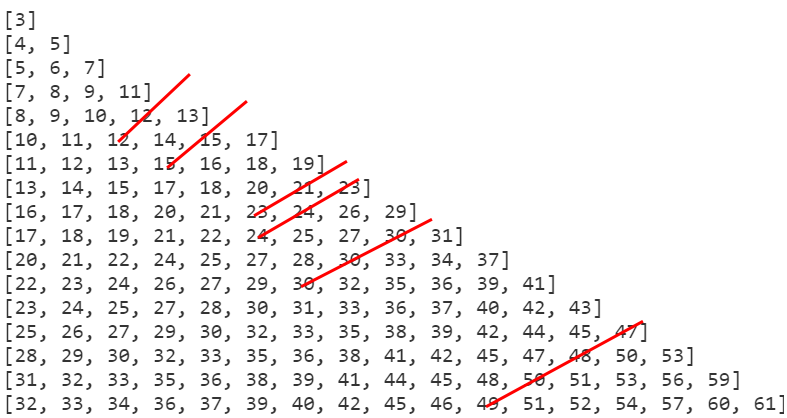
\includegraphics[]{20230830conclusion1.png}
		\caption{In GT, the left part of red line appears as continuous integers}
		\label{fig:conclusion1}
	\end{figure}
	\begin{proof}
		This statement is roughly equivalent to \eqref{GoldbachConjectureInequality2}
	\end{proof}

	\begin{proposition}[Conclusion 2]
		\begin{enumerate}
			\item The sequence of numbers on each vertical line, horizontal line, 
			and backslash line($\diagdown$) in Goldbach triangle is strictly 
			increasing since primes are increasing. Furthermore, the 
			intersection of any two adjacent backslash lines ($\diagdown \diagdown$)must be empty. 
			\item When the number of rows in Goldbach triangle is sufficient, 
			the two sequences on any two non-adjacent backslash lines ($\diagdown..\diagdown$) must have a non-empty intersection. 
			\item Except $\{3\}, \{4\}, \{5, 5\}, \{7, 6\}$ at the beginning of Goldbach triangle, 
			each sequence of forward slash lines (/) must have repeated values, such as \\
			$\{8,8,7\}, \{10,9,9\},\{11,11,10,11\},\cdots$
		\end{enumerate}		
	\end{proposition}

	\begin{proposition}[Conclusion 3]
		when $n>2$, $det(\text{PSDM}_n)==0$
	\end{proposition}
	\begin{table}[h]
		\caption{odd Primes Semi-Distance Matrix PSDM7}
		\label{table:2}
		\begin{tabular}{lllllll}
		0 & -1 & -2 & -4 & -5 & -7 & -8 \\
		1 & 0  & -1 & -3 & -4 & -6 & -7 \\
		2 & 1  & 0  & -2 & -3 & -5 & -6 \\
		4 & 3  & 2  & 0  & -1 & -3 & -4 \\
		5 & 4  & 3  & 1  & 0  & -2 & -3 \\
		7 & 6  & 5  & 3  & 2  & 0  & -1 \\
		8 & 7  & 6  & 4  & 3  & 1  & 0 
		\end{tabular}
	\end{table}








\clearpage
%\onehalfspacing
\bibliographystyle{plain}
\bibliography{main}
\addcontentsline{toc}{section}{References}

\end{document}